
\begin{activity} \label{A:9.1.9}
\begin{figure}[ht]
\begin{center}
%\resizebox{!}{1.75in}{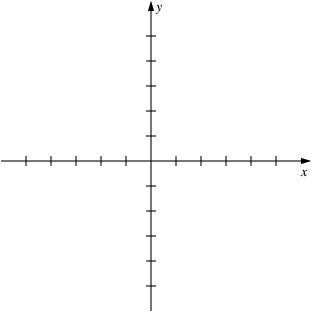
\includegraphics{figures/9_1_contour_activity_1}} 
%\hspace{0.2in} 
%\resizebox{!}{1.75in}{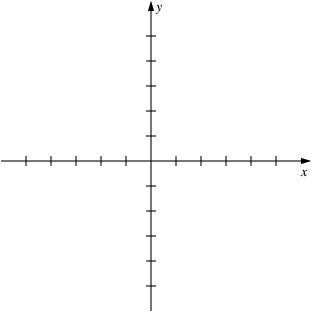
\includegraphics{figures/9_1_contour_activity_1}}
  \includegraphics{figures/fig_9_1_activity_empty_1.eps}
  \hspace*{0.5in}
  \includegraphics{figures/fig_9_1_activity_empty_2.eps}
\caption{Left: Level curves for $f(x,y) = x^2+y^2$. Right: Level curves for $g(x,y) = \sqrt{x^2+y^2}$.}
\label{F:9.1.contour_activity}
\end{center}
\end{figure}
   \ba
    \item Let $f(x,y) = x^2+y^2$. Draw the level curves $f(x,y) = k$ for $k=1$, $k=2$, $k=3$, and $k=4$ on the left set of axes given in Figure \ref{F:9.1.contour_activity}. (You decide on the scale of the axes.) Explain what the surface defined by $f$ looks like.

    \item Let $g(x,y) = \sqrt{x^2+y^2}$. Draw the level curves $g(x,y) = k$ for $k=1$, $k=2$, $k=3$, and $k=4$ on the right set of axes given in Figure \ref{F:9.1.contour_activity}. (You decide on the scale of the axes.) Explain what the surface defined by $g$ looks like.

    \item Compare and contrast the graphs of $f$ and $g$. How are they alike? How are they different? Use traces for each function to help answer these questions.

     \ea

\end{activity}
\begin{smallhint}
\ba
\item The contours have graphs that should be familiar. 
\item The contours have graphs that should be familiar.
\item How well spaced are the contours of $f$ and $g$?  
\ea
\end{smallhint}
\begin{bighint}
\ba
\item What familiar graph does the equation $x^2+y^2=1$ have?
\item What equation do you get if you square both sides of $1 = \sqrt{x^2+y^2}$?
\item What kind of graph is $y=x^2+C$ where $C$ is a constant? What kind of graph if $y = \sqrt{x^2}$? 
\ea
\end{bighint}
\begin{activitySolution}
\ba
\item The contours of $f$ are shown at left in the figure below.  The contours are circles, getting closer together as we move away from the origin, indicating a graph that is increasing quickly as we move away from the origin in all directions. The surface defined by $f$ looks like a bowl anchored at the origin that opens up. %Figure \ref{F:9.1.contour_activity_sol}.
\item The contours of $g$ are shown at right in the figure below. The contours are circles that appear to be uniformly spaced as we move away from the origin. This indicates that the surface defined by $g$ looks like a cone anchored at the origin that opens up. %Figure \ref{F:9.1.contour_activity_sol}. 
    \item The contours of $g$ are more uniformly spaced as we move away from the origin than those  in part (a). So we should expect the graph of $f$ to increase more rapidly as we move radially from the origin than the graph of $g$. To see this in another light, the traces of $f$ for fixed $y$ have the form $z = k^2+x^2$ for constants $k$, which are parabolic in form. By symmetry, the traces of $f$ for fixed values of $x$ have the same shape. By contrast, the traces of $g$ for fixed $y$ have the form $z = \sqrt{k^2+x^2}$ for constants $k$. In particular, the trace with $k=0$ has the form $z = \sqrt{x^2} = | x |$, which is linear. By symmetry, the traces for fixed $y$ have the same shape. This confirms our statements in (a) and (b) that the graph of $f$ is parabolic (bowl shaped), while the graph of $g$ looks like a cone. 
    \ea
%\begin{figure}[ht]
\begin{center}
\resizebox{!}{1.75in}{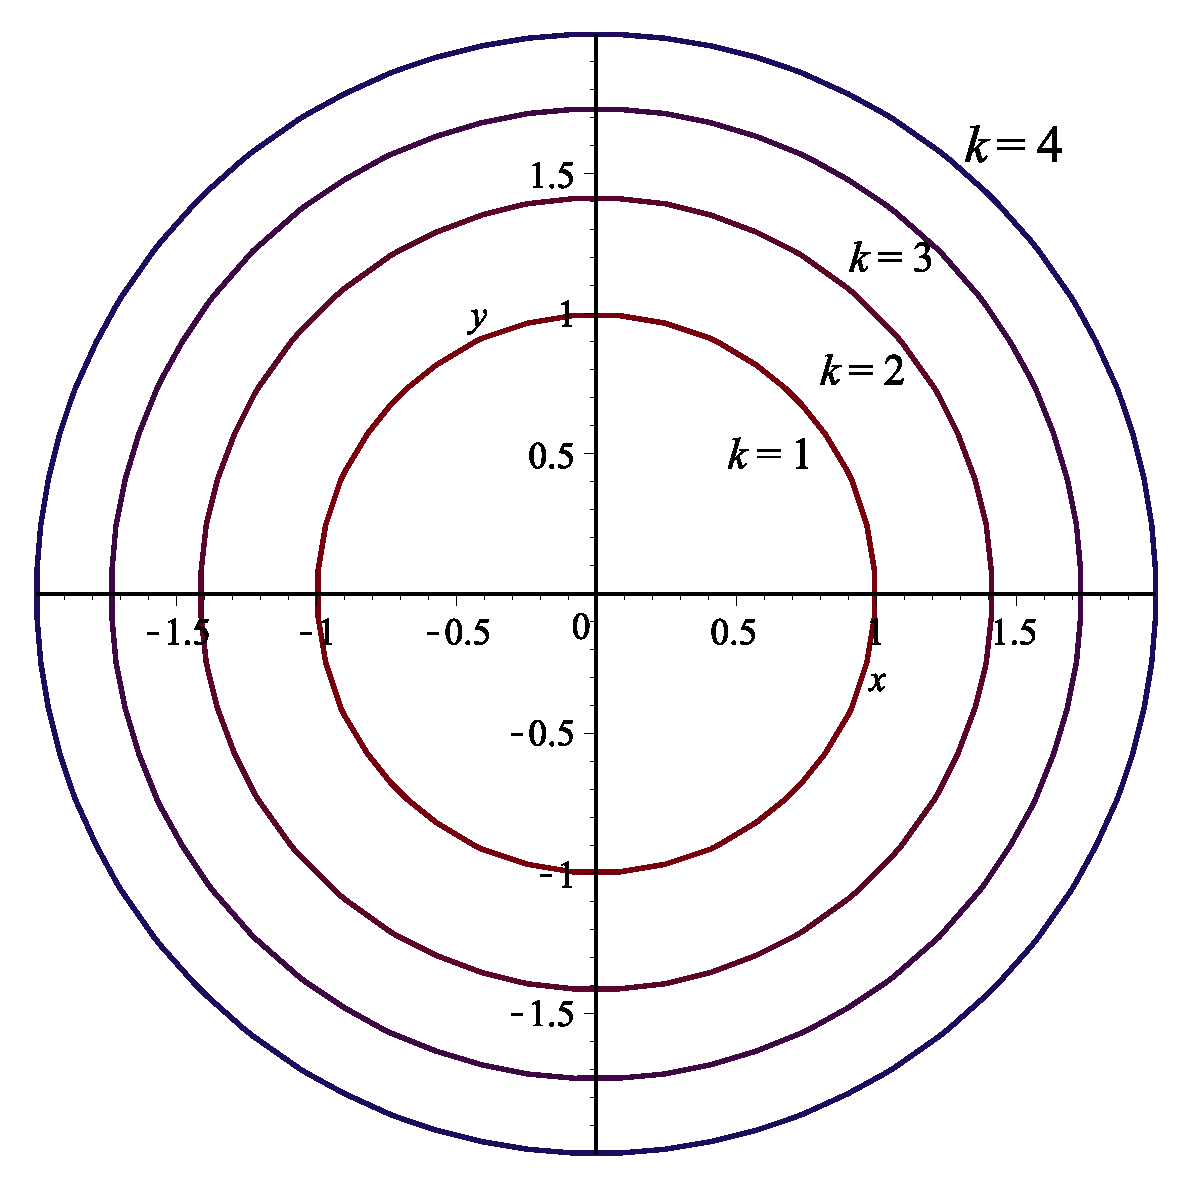
\includegraphics{figures/9_1_contour_activity_1a}} \hspace{0.2in} \resizebox{!}{1.75in}{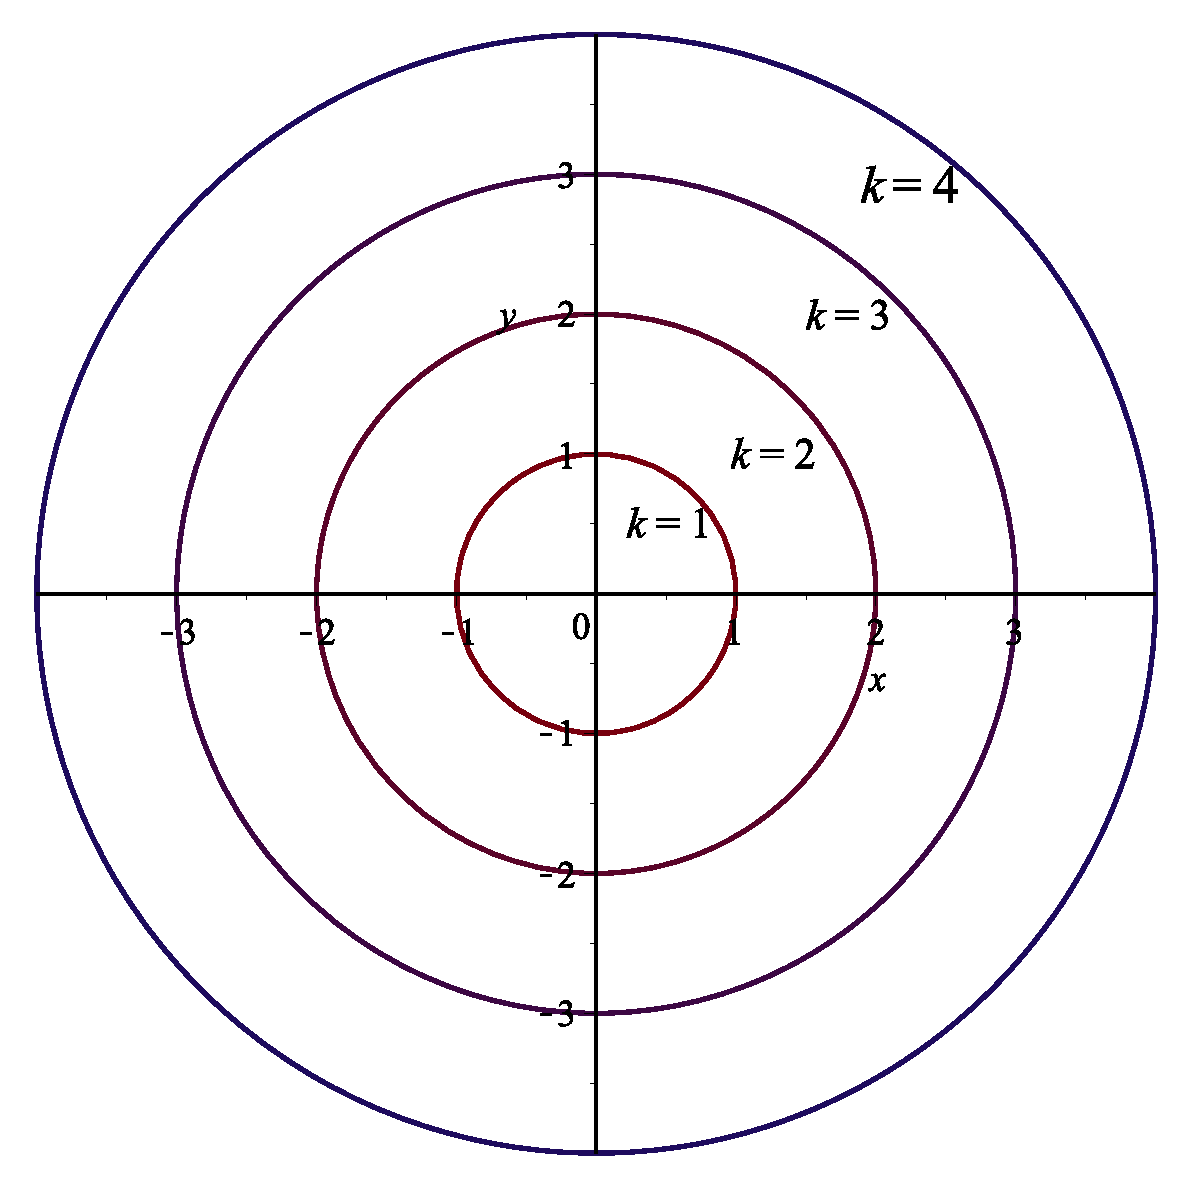
\includegraphics{figures/9_1_contour_activity_1b}}
%\caption{Left:Level curves for $f(x,y) = x^2+y^2$. Right: Level curves for $g(x,y) = \sqrt{x^2+y^2}$.}
%\label{F:9.1.contour_activity_sol}
\end{center}
%\end{figure}
\end{activitySolution}


\aftera 